\chapter{Kehitysympäristö}

\section{Ongelma}
Yleisin ongelma usean kehittäjän tiimissä on kehitysympäristön erilaisuus. Tämä ilmenee parhaiten kun kehittäjät käyttävät työkoneellaan eri käyttöjärjestelmiä kuten Linuxia, OS X:ää ja Windowsia. Usein projekteissa on pitkät asennusohjeet, jossa kerrotaan tarkasti mitkä riippuvuudet pitää asentaa sekä niiden tarkat versionumerot. Usein riippuvuuksien asennus on erilaista riippuen käyttöjärjestelmästä. Ei ole epätavallista, että ympäristön pystytykseen voi mennä muutama työpäivä. Oman kokemukseni mukaan pystytysprosessiin menee paljon henkilötyötunteja, sillä lähes aina tarvitaan apua projektissa aikaisemmin olleelta henkilöltä.

\section{Ratkaisu}
Jotta kaikille kehittäjille saadaan täysin samanlaiset kehitysympäristöt niin yksi ratkaisu on virtuaalikoneet. VirtualBox tai WMware ovat esimerkkejä virtuaalikoneohjelmista. Virtuaalikoneet ovat täysiverisiä käyttöjärjestelmiä isäntäkoneen eli käyttäjän koneen sisällä. Usein kehityskäyttöjärjestelmäksi valitaan jokin Linux paketti esimerkiksi Ubuntu. Näin kaikille kehittäjille saadaan sama käyttöjärjestelmä, jossa kehitys tapahtuu. Tämä vähentää riippuvuuksien asentamisessa tapahtuvaa virheiden määrää.

Pelkkä käyttöjärjestelmän yhdenmukaistaminen ei riitä sillä riippuvuuksien asentamisessa yleensä ongelmat ilmenevät. Pelkkä VirtualBox ei riitä sillä kaikki siihen halutut ohjelmat pitää asentaa käsin tai tehdä iso kokoinen levykuva, josta asennettaisiin ympäristö.

\section{Vagrant}
Vagrantin avulla voidaan luoda virtuaalikoneita helposti komentoriviltä. Vagrant on yksinkertainen ohjelma, joka vain käskyttää VirtualBoxia. Tästä syystä VirtualBox täytyy olla asennettuna, jotta Vagrant toimii.

Vagranttia kannattaa ajatella vertauskuvan kautta. Kuvitellaan, että Erik haluaa perustaa Subway-ravintolan. Koska Subway on pikaruokaravintolaketju sillä on tarkasti määritelty mitä aineksia ruoka-annoksissa saa käyttää, minkälaiset työvaatteet pitää olla ja miten asiakaspalvelu pitäisi toimia tms. Erik saa itse valita tilan johon perustaa ravintolan. Tilan valitsemisen jälkeen hänen täytyy sisustaa ravintola Subwayn määrittämällä tavalla. Seuraavaksi täytyy hankkia uuni, jääkaappi, mikro ja muut ruuan tekemiseen tarkoitetut välineet. Tässä vaiheessa saattaa tulla tilanne, jossa kaikki hankitut laitteet eivät välttämättä sovi valittuun liiketilaan. Esimerkiksi Erikin valitsemalle jääkaappille ei löydy sopivaa paikkaa liiketilasta. Paljon yhteensopivuus ongelmia voi syntyä ennen kuin uusi Subway-ravintola voidaan avata. Tämä on luonnollista, koska Subwayn johto ei voi tietää miten kaikki laitteet menevät mihin tahansa liiketilaan.

Kun Subwayn liikejohto huomasi, että uusilla ravintoloiden perustajilla on usein ongelmia ravintolan pystyttämisessä ja sen saamiseksi ohjeiden mukaiseen kuntoon he päättivät helpottaa asiaa. He kehittivät uusien ravintoloiden perustajille paketin, josta täytyy vain painaa nappia eikä ravintoloitsijan tarvitse tehdä muuta. Erik kokeili uutta asennuspakettia ja huomasi, että paketista tuli ulos robotti, joka lähti heti rakentamaan liiketilaa ravintolalle. Robotti rakentaa aina samanlaisen tyhjän liiketilan johdon määrittelemällä tavalla. Kun liiketila on valmis robotti aloittaa jääkaappien, uunien ja muiden laitteiden asentamisen, jotka ovat välttämättömiä Subway-ravintolan pitäjälle. Kun laitteet ovat asennettu liiketila viimeistellään sisustuksella. Robotti tiesi miten asennukset ja sisustaminen pitää tehdä, koska sille on määritelty ohje, jota se lukee. Kun robotti on tehnyt kaiken se antaa liiketilan avaimet Erikille, jonka ei tarvitse muuta kuin laittaa uunit päälle niin hän voi aloittaa myymisen.

\subsection{Vagrantin toiminta}
Vagrant luo isäntäkoneen sisälle virtuaalikoneen kuten kuvassa \ref{fig:how-vagrant-works}.Virtuaalikone sisältää kaikkille kehittäjille yhteinen käyttöjärjestelmän. Lisäksi Vagrantille annetaan "resepti", jonka mukaan se asentaa kaikki projektin riippuvuudet. Koodin kääntäminen, komentojen ajaminen, mahdollisen tietokannan käyttäminen tms. asiat tehdään virtuaalikoneella. Näin isäntäkone pysyy puhtaana turhista ohjelmista, eikä synny aikaisemmin mainittuja ongelmia. Isäntäkoneessa tapahtuu koodin kirjoittaminen, tiedostojen luonti ja versiohallinan käyttäminen.

\begin{figure}[h]
  \includegraphics[width=\textwidth]{how-vagrant-works}
  \caption{Vagrantin toiminta isäntäkoneen sisällä}
  \label{fig:how-vagrant-works}
\end{figure}

\subsection{Vagrantin käyttäminen}
Ennen Vagrantin käytön aloittamista täytyy VirtualBox ja Vagrant olla asennettuna. Avaamalla terminaalin voit nyt käyttää vagrant-komentoja terminaalissa. Jos komento \code{vagrant -v} palauttaa Vagrantin nykyisen version niin asennus on mennyt oikein. Tästä eteenpäin työskennellään koko ajan terminaalissa.

Siirry projektikansioon ja aja \code{vagrant init}. Vagrant luo kansioon Vagrantfile-nimisen tiedoston. Vagrantfile on käytännössä Ruby-ohjelmointi kieltä, jota Vagrant osaa lukea kun se ajetaan. Vagrantfilessä voi siis käyttää kaikkia Ruby-kielen toimintoja. Kuviosta \ref{listing:InitialVagrantfile} näkyy tiedoston sisältö ilman kommentteja.

\begin{lstlisting}[
  label=listing:InitialVagrantfile,
  language=Ruby,
  caption=Alustava Vagrantfile,
  float=h
]
Vagrant.configure(2) do |config|
  config.vm.box = "ubuntu/trusty64"
end
\end{lstlisting}

Kaikki virtuaalikoneen asetukset tulevat config-osion sisälle. Tällä hetkellä koneelle määritellään vain boxi: "ubuntu/trusty64". Mahdollisia boxeja voi etsiä osoitteesta: \url{https://atlas.hashicorp.com/boxes/search}. Boxit ovat käytännössä käyttöjärjestelmä eli pohja virtuaalikoneelle. Tässä tapauksessa boxina on Ubuntu, joka perustuu Debian Linux-jakeluun \cite{link:ubuntu}. Boxi on ravintolavertauskuvassa ravintolan liiketila. Boxi on pakko olla, mutta itsessään sillä ei tee paljon mitään. Boxi täytyy "sisustaa" eli asentaa projektiin liittyvät ohjelmat ja riippuvuudet.

Yksinkertaisin keino asentaa ohjelmia virtuaalikoneelle on shell-skriptien avulla. Jos projektiin tarvitsee asentaa vain muutama ohjelma voidaan ne asentaa laittamalla asennus-skripti suoraan Vagrantfileen. 

\begin{lstlisting}[
  label=listing:vagrant-shell-inline,
  language=Ruby,
  caption=Vagrantin yksinkertainen shell-skripti,
  float=h
]
config.vm.provision "shell",
  inline: "apt-get update; apt-get install -y apache2"
\end{lstlisting}

Kuviossa \ref{listing:vagrant-shell-inline} Vagrantfilen sisään on lisätty provisiointi shell-skripti, joka on tyyppiä inline. Tällä tarkoitetaan, että koko skripti annetaan suoraan stringinä. Tässä esimerkissä \code{apt-get update} päivittää virtuaalikoneen lokaalitpaketti linkit. \code{apt-get install -y apache2} tarkoittaa että asennetaan Apache-palvelinohjelma, jota monet käyttävät esimerkiksi PHP-projekteissa. Lippu -y pitää lisätä, koska apt varmistaan usein käyttäjältä, että haluaako hän varmasti asentaa kyseisen paketin. Lippu varmistaa sen, että kaikki pakettiin liittyviin kysymyksiin vastataan kyllä.

Skripti voidaan myös jakaa monelle riville Rubyn HEREDOC:n avulla kuvion \ref{listing:vagrant-shell-heredoc} osoittamalla tavalla. HEREDOC \cite{link:ruby-heredoc} mahdollistaa stringin kirjoittamisen monelle riville, mikä helpottaa luettavuutta kun asennetaan paljon ohjelmia.

\begin{lstlisting}[
  label=listing:vagrant-shell-heredoc,
  language=Ruby,
  caption=Vagrantin shell-skripti HEREDOC:lla,
  float=h
]
config.vm.provision "shell", inline: <<-SHELL
  apt-get update
  apt-get install -y apache2
SHELL
\end{lstlisting}

Käytännössä kuitenkin shell-skripti kannattaa laittaa erilliseen tiedostoon kuten kuviossa \ref{listing:vagrant-shell-path}. Jos Vagrantfile ja shell-skripti ovat samassa kansiossa niin riittää kun laittaa vain skriptin nimen.

Ulkoiseen skriptii täytyy laittaa alkuun kommentti, jossa kerrotaan, että kyseessä on shell-skripti. Ulkoisen skriptiin on helppo määritellä paljon eri ohjelmien asennuksia ja konfigurointeja.

\begin{lstlisting}[
  label=listing:vagrant-shell-path,
  language=Ruby,
  caption=Provisiointi-skripti voi olla myös erillisessä tiedostossa,
  float=h
]
config.vm.provision "shell", path: "install-environment.sh"
\end{lstlisting}

\begin{lstlisting}[
  label=listing:vagrant-external-shell-script,
  language=bash,
  caption=Ulkoinen shell-skripti,
  float=h
]
#!/bin/bash
apt-get update
apt-get install -y apache2
\end{lstlisting}

Koska projektin koodaaminen tehdään host-koneella niin haluamme saada yhteyden esimerkiksi Apache-palvelimeen suoraan host-koneelta. Siksi seuraavaksi pitää avata virtuaalikoneen portteja host-koneelle. Apache vastaa oletuksena osoitteesta \url{http://localhost:80}, joten haluamme avata portin 80 isäntäkoneelle. Vagrantfileen voidaan määrittää mikä virtuaalikoneen portti halutaan ohjata mihin isäntäkoneen porttiin. Kuviossa \ref{listing:vagrant-port-mapping} virtuaalikoneen portti 80 ohjataan isäntäkoneen porttiin 8080.

\begin{lstlisting}[
  label=listing:vagrant-port-mapping,
  language=Ruby,
  caption=Virtuaalikoneen portti 80 ohjataan isäntäkoneen porttiin 8080,
  float=h
]
config.vm.network "forwarded_port", guest: 80, host: 8080
\end{lstlisting}

Nyt kun isäntäkoneella mennään selaimella osoitteeseen \url{http://localhost:8080} niin pitäisi tulla näkyviin Apachen oletussivu jos Apache on asennettu joillakin edellä mainituilla tavoilla virtuaalikoneeseen. Kuvassa \ref{fig:apache-default-page} näkyy Apachen oletussivu kun virtuaalikoneen portit on ohjattu oikein.

\begin{figure}[h]
  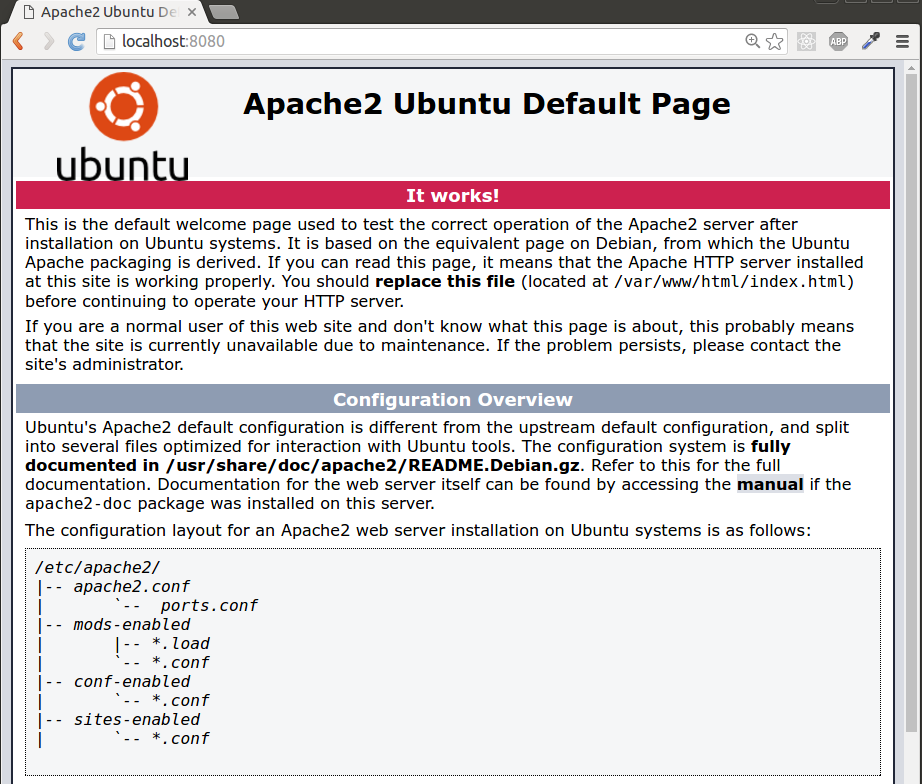
\includegraphics[width=\textwidth]{apache-default-page}
  \caption{Isäntäkone näkee Apachen oletussivun kun oikeat portit ovat auki}
  \label{fig:apache-default-page}
\end{figure}

Nyt kun Apache on asennettu oikein voidaan viedä virtuaalikoneelle projektin tiedostostot. Oletetaan, että projektissa on yksinkertaisuuden vuoksi vain index.html-tiedosto. Kuviossa \ref{listing:vagrant-synced-folder} näytetään miten haluttu kansio saadaan synkronoitua virtuaalikoneeseen.

Ensimmäinen parametri kertoo mikä isäntäkoneen kansio halutaan synkronoida. Polun voi antaa relatiivisena tai absoluuttisena. Tässä tapauksessa parametri on relatiivisesti nykyinen kansio. Toinen parametri kertoo minne kansio halutaan synkronoitua virtuaalikoneessa. Isäntäkoneen kansio halutaan synkronoida kansioon /var/www/html, koska sieltä Apache lukee oletuksena tiedostoja. Nyt kun lisätään projektin juureen isäntäkoneella tiedosto index.html, jonka sisältönä on \code{Hello from project file} saadaan kuvan \ref{fig:index-file-response} mukainen vastaus Apachelta.

\begin{figure}[h]
  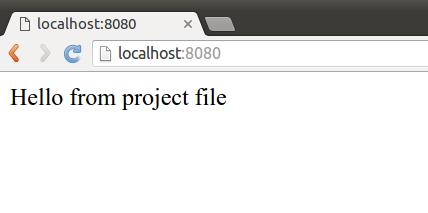
\includegraphics[width=\textwidth]{index-file-response}
  \caption{Apache vastaa index.html tiedoston sisällön}
  \label{fig:index-file-response}
\end{figure}

Vagrant synkronoi tiedostot valittujen kansioiden välillä molempiin suuntiin. Kun tiedosto lisätään isäntäkoneella niin sama tiedosto ilmestyy virtuaalikoneelle. Samoin jos virtuaalikoneelle lisätään tiedosto synkronoituun kansioon niin tämä tiedosto tulee isäntäkoneelle. Työskennellessä on kuitenkin tarkoitus toimia lisäämällä tiedostoja aina isäntäkoneelle.


Jos isäntä- ja virtuaalikoneella on kaksi saman nimistä tiedostoa niin isäntäkoneella oleva tiedosto ylikirjoittaa virtuaalikoneen tiedoston. Esimerkiksi kansiossa /var/www/html on Apachen oletus index.html-tiedosto, mutta projektin index.html ylikirjoittaa sen.

Kuvassa \ref{fig:how-vagrant-works} on visualisoitu kaksisuuntainen kansion synkronointi.

\begin{lstlisting}[
  label=listing:vagrant-synced-folder,
  language=Ruby,
  caption=Isäntäkoneen kansio synkronoidaan virtuaalikoneen kansioon,
  float=h
]
config.vm.synced_folder ".", "/var/www/html"
\end{lstlisting}

Vagrantin hyödyt
\begin{bullet-list}
  \item Ei tarvitse omalle (hosti)koneelle asentaa mitään.
  \item Projektin ympäristön asennustiedot ovat version hallinnassa Vagrantfilessä ja shell-skripteissä.
  \item Ympäristön saa pystyyn vain komentamalla \code{vagrant up}.
  \item Kaikilla kehittäjillä sama ympäristö.
\end{bullet-list}

Vagrantin haitat
\begin{bullet-list}
  \item Virtuaalikoneet vievät välillä enemmän keskusmuistia kuin lokaalisti ajaessa.
  \item Yleensä tarvitsee tehdä lisäsäätöä esimerkiksi ku tarkkaillaan tiedoston muutoksia.
\end{bullet-list}

\subsection{Alaluvun alaotsikko}

Otsikon jälkeen tulee tekstiä tai uusi alaotsikko.

\begin{table}[h]
  \caption{Metropolian opiskelijoiden lukuvuonna 2009–2010 suorittamat virtuaaliopinnot.}
  \begin{tabular}{| l | l | l |}
  \hline
  \bfseries Koulutusala & \bfseries Suoritusten määrä, op \\
  \hline
  Kulttuuriala & 131 \\
  \hline
  Tekniikan ja liikenteen ala & 552 \\
  \hline
  Sosiaali- ja terveysala & 175 \\
  \hline
  Liiketaloudena ala & 52 \\
  \hline
  Ei sidottu koulutusalaan & 18 \\
  \hline
  \bfseries Metropolia yhteensä & \bfseries 928 \\
  \hline
  \end{tabular}
  \label{tab:virtual studies}
\end{table}

Kuvan tai taulukon jälkeen tulee tekstiä ennen uutta kuvaa tai taulukkoa tai seuraavaa otsikkoa.

\subsection{Alaluvun alaotsikko}

Alaluvun alaotsikon jälkeen tulee tekstiä.

Sitaatti toteutetaan Lainaus-tyylillä. Sitaatin johtolauseen sisältävässä kappaleessa (välittömästi sitaattia edeltävässä kappaleessa) käytetään tyyliä ”Leipäteksti ennen lainausta”, jotta sitaatin ja johtolauseen väliin jää lyhyempi kappaleväli.

\begin{quote}
Usean rivin pituinen suora lainaus kirjoitetaan kirjainkoolla 10. Tekstissä käytetään riviväliä 1, ja teksti sisennetään. Suorassa lainauksessa käytetään mallipohjan lainaustyyliä. Lainaukseen merkitään lähdeviite.
\end{quote}